\chapter{Model Specification}
\label{chap:1} 
In this chapter we describe the abstract models used to shape all the three parts of the system from a geometric perspective. (FARE QUI UN ELENCO? torretta, puntamento, relloc)
\section{Turret Model}
\label{sec:1.1}
Degree of Freedom (DoF) is the number of independent parameters that define the configuration of a mechanical system. In our case, we wanted to build a two DoF Pan \& Tilt turret. That means that our parameters are two angles. In a 3D reference system, \textbf{pan} is the horizontal angle about the upright Z axis, \textbf{tilt} is the vertical angle about the rotated Y axis, as in figure \ref{fig:panTilt}.
Our final goal is to be able to define the direction of a laser ray mounted on top of the turret, so that we can control the position of the projected laser dot on a given surface, by solving the system's inverse kinematics.\\
\begin{figure}
	\centering
	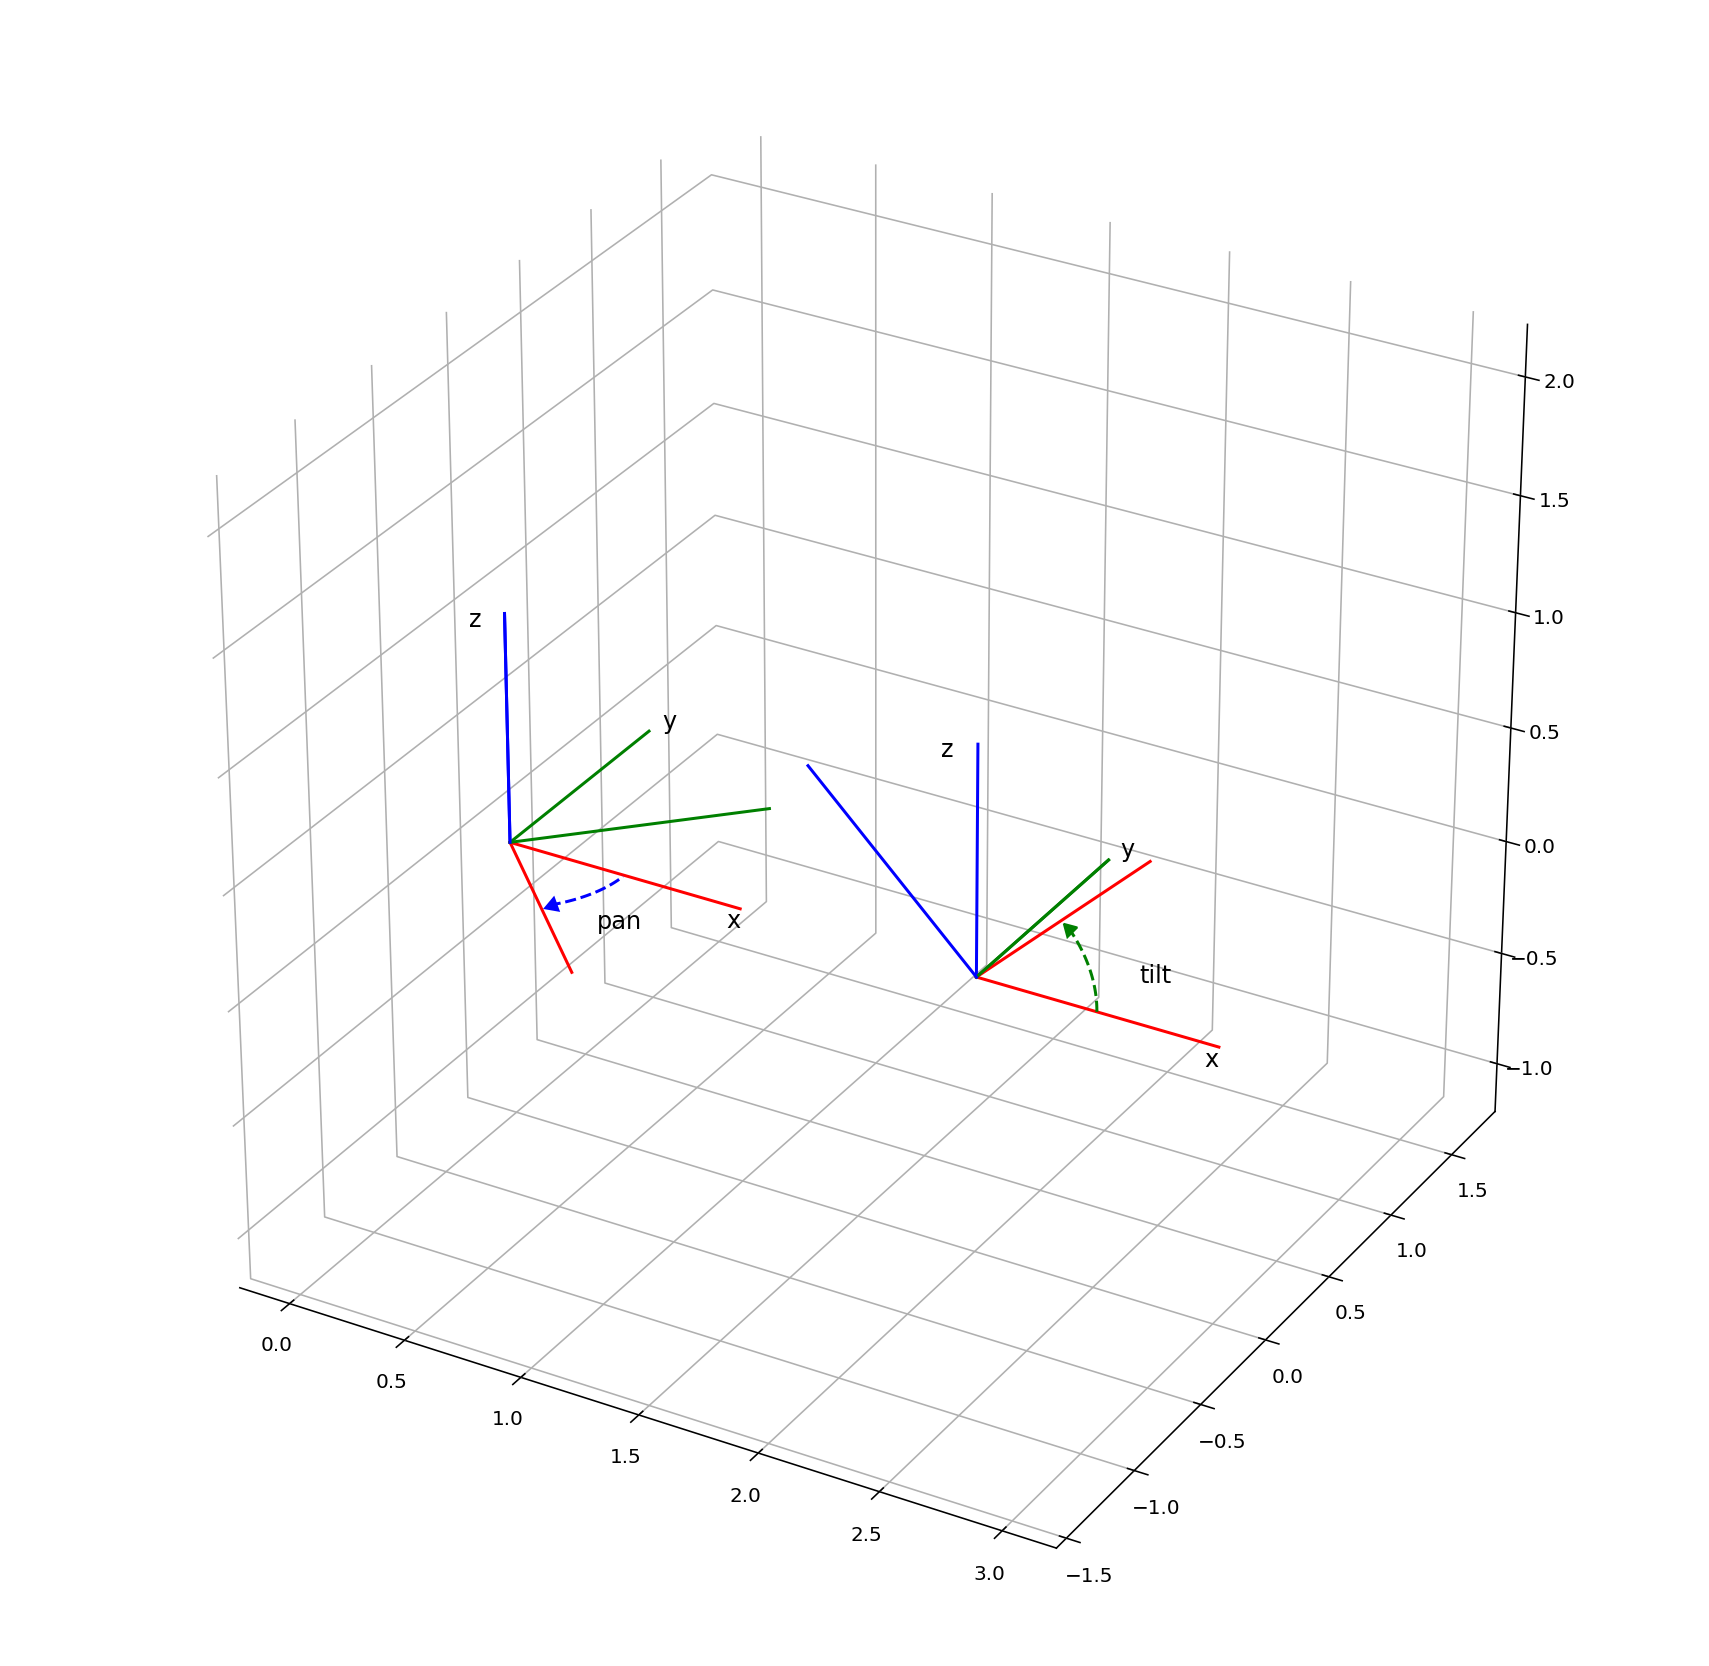
\includegraphics[width=\textwidth]{img/panTilt.png}%
	\caption{Pan and Tilt}
	\label{fig:panTilt}
\end{figure}
For those purposes, we have built two different turrets. Since the model of the first one is slightly simpler than the second, we will start describing the former, which turns out to be helpful to understand the latter. We will focus on the case in which the laser must be projected on the ground.

\subsection{First Model}\label{subs:firstModel}
First, figure \ref{fig:firstModelRefFrame} helps us understand how we have shaped the model to match the physical structure of the turret. We have three reference frames. The \textbf{base\_frame} is fixed and is the one in which we define the coordinates of the projected point. \textbf{pan\_frame} and \textbf{tilt\_frame} are the frames used to represent our revolute joints.
\textbf{H} is the height of the turret, which is known. Note that the convention used for the frame is the following:
\begin{itemize}
    \item red is the x axis;
    \item green is the y axis;
    \item blue is the z axis.
\end{itemize}
Thus, we consider the laser ray to be a prolongation of the x axis of the \textbf{tilt\_frame}. \\
Figure \ref{fig:firstModelPanTilt} shows what we want to be able to do: given the \textit{x}, \textit{y} and \textit{z} of the laser point we want to set \textbf{pan} and \textbf{tilt} angles accordingly. In order to do so, firstly we will solve the forward kinematic, then the inverse will be easily derived.
\subsubsection{Forward Kinematic}
The forward kinematic should take as input our parameters (i.e. \textbf{pan} and \textbf{tilt}) and then return the coordinates of the laser projected point into \textbf{base\_frame} reference. 
Note that, since we are controlling the direction of an infinite ray, in order to obtain a unique (\textit{x, y, z}) triple, we must intersect such ray with a plane defined by the triple (\textit{0, 0, z}). In the forward kinematic equations this can be obtained by assuming that we know the \textit{z} of the point we want. Another option could be to assume that \textit{z} is zero, since we are considering the laser projection on the floor (i.e. on the \textbf{base\_frame}). \\
As well as what is already defined in figure \ref{fig:firstModelPanTilt}, we must add:
\begin{itemize}
    \item \textbf{L} as the distance from the \textbf{pan\_frame} origin to the projection of the laser point on the \textbf{base\_frame};
    \item \textbf{D} as the distance from the \textbf{tilt\_frame} origin to the laser point.
\end{itemize}
First, note that the \textbf{pan} angle does not depends on the \textit{z} coordinate, so, starting from:
\begin{align}
	D=& \frac{H-z}{\cos{(tilt)}} \label{eq:d}\\
	L=& \sqrt{(H-z)^2 + D^2}
\end{align}
We can easily obtain laser point coordinates:
\begin{align}
	x=& L\cos{(pan)}\label{eq:x}\\
	y=& L\sin{(pan)} \label{eq:y}
\end{align}

\begin{figure}
	\centering
	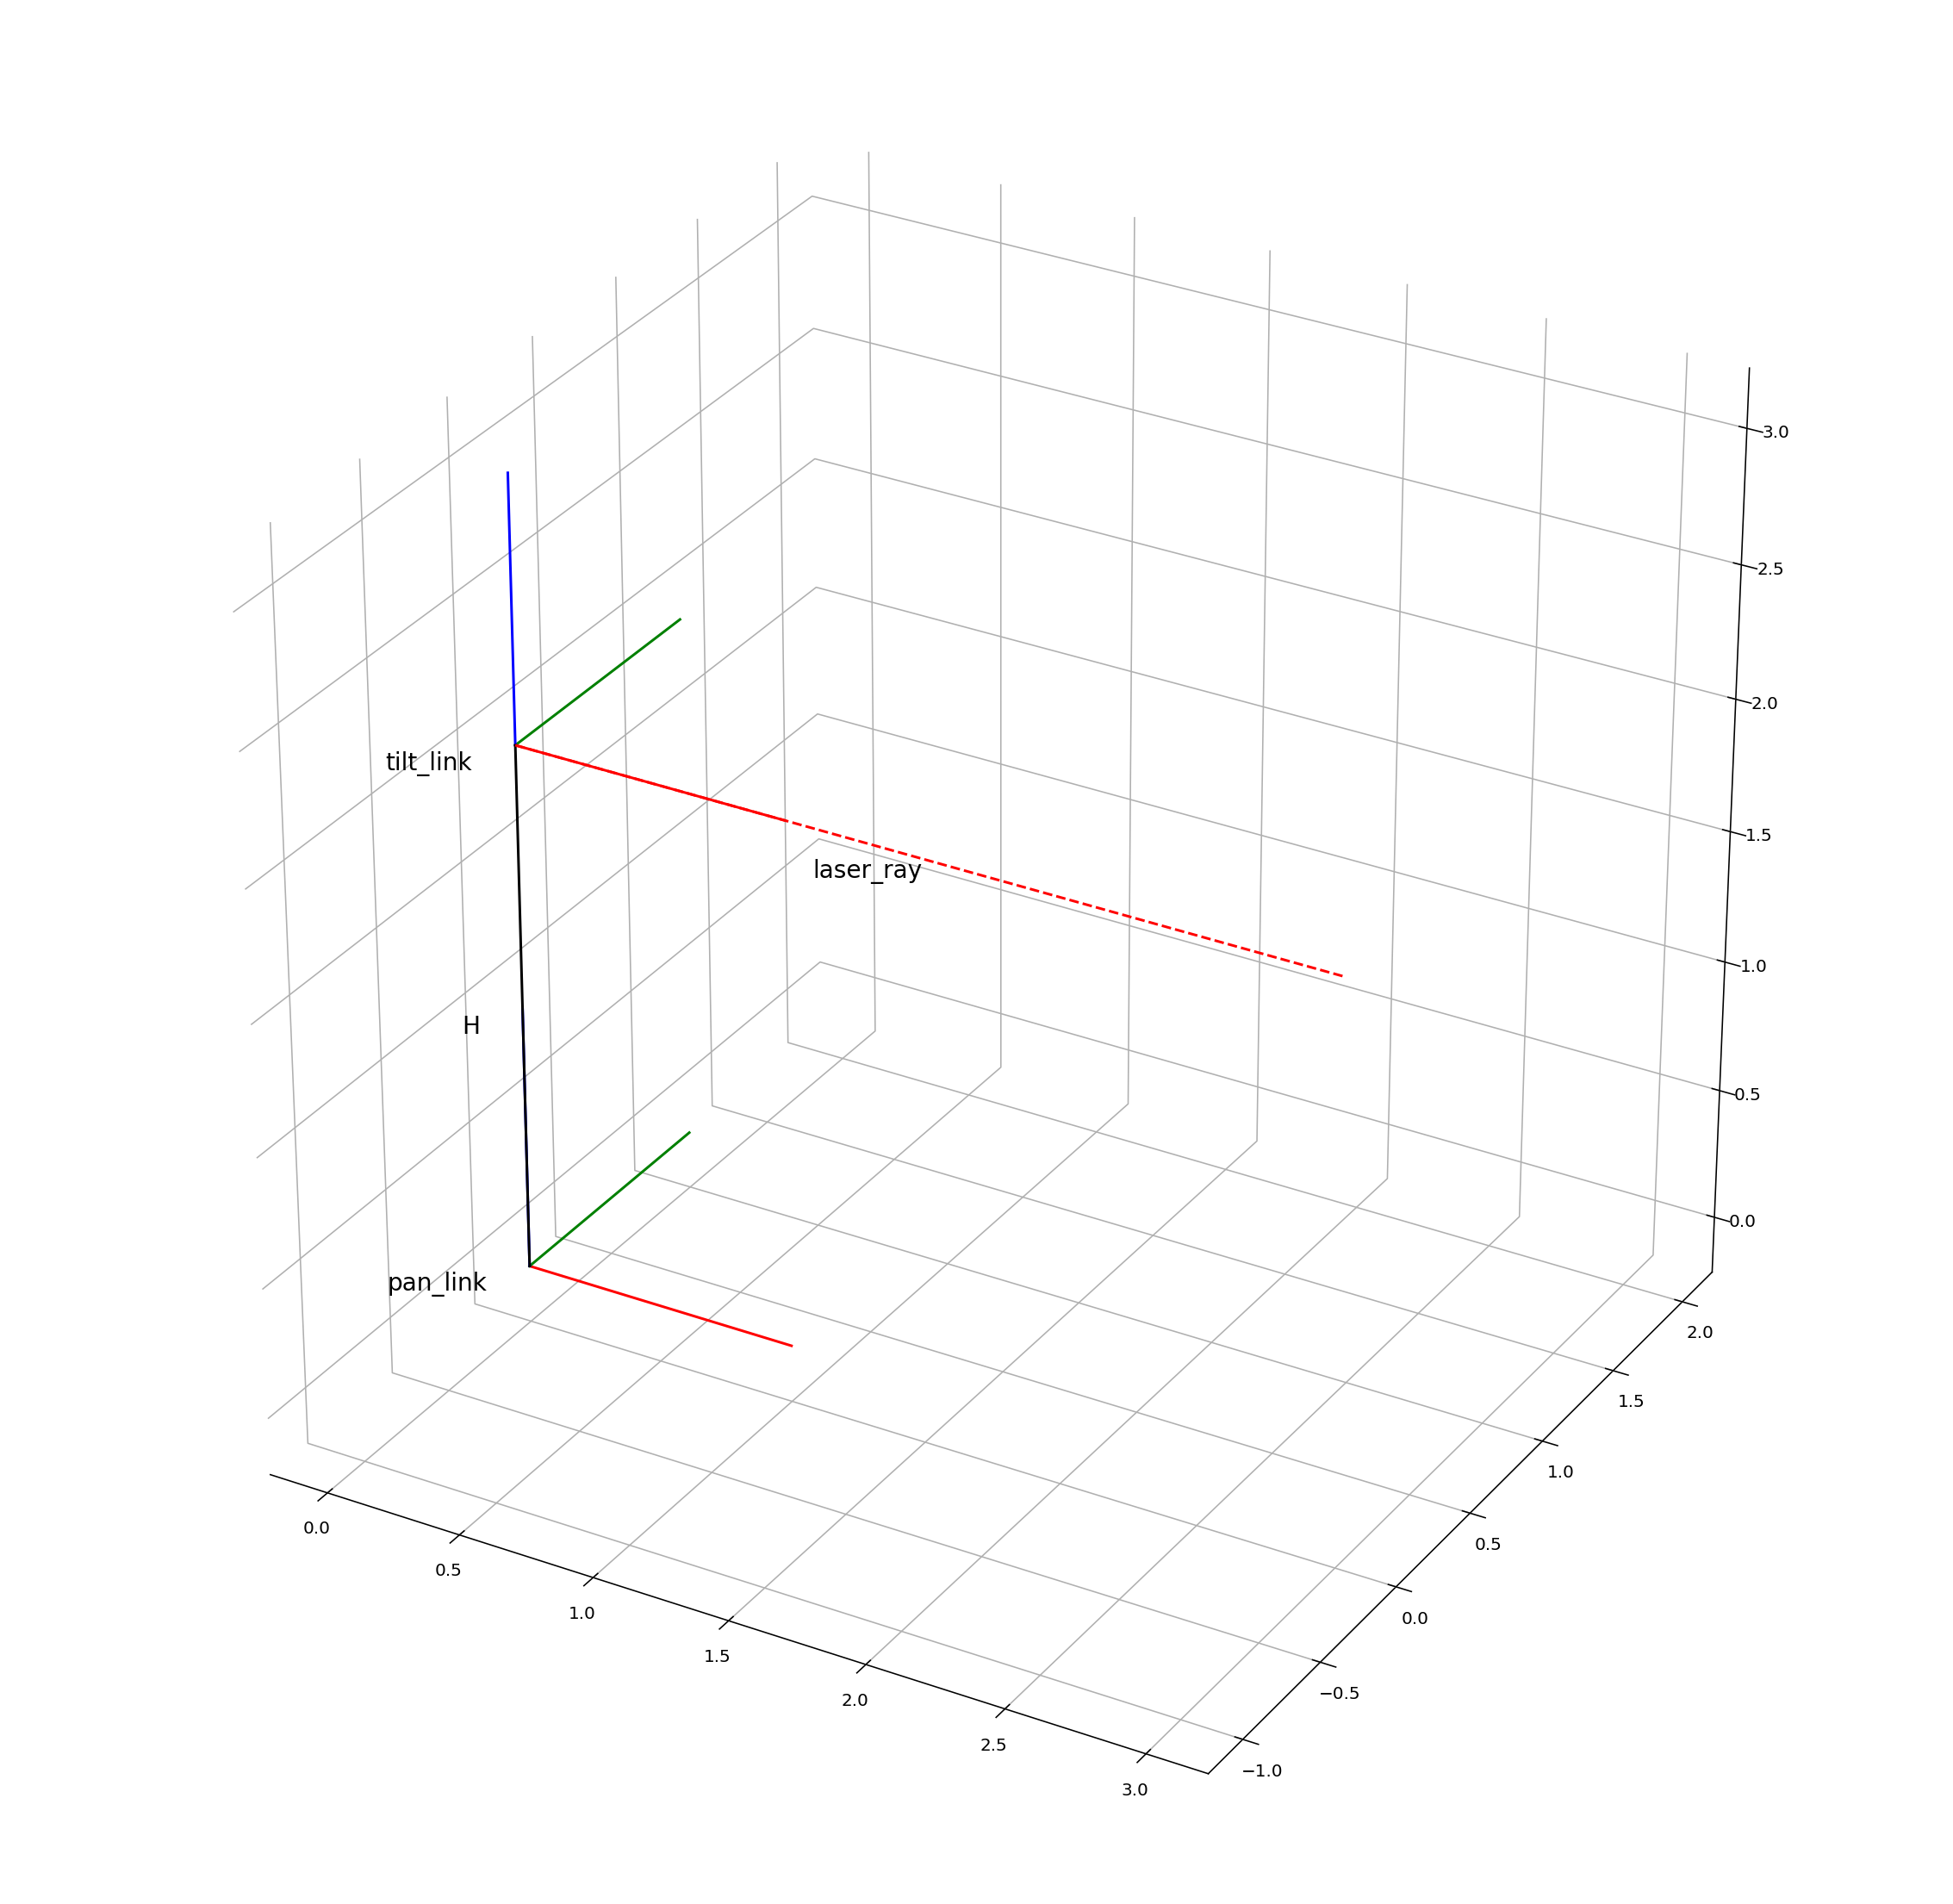
\includegraphics[width=\textwidth]{img/firstModel.png}%
	\caption{First Model, Reference Frames}
	\label{fig:firstModelRefFrame}
\end{figure}
\begin{figure}
	\centering
	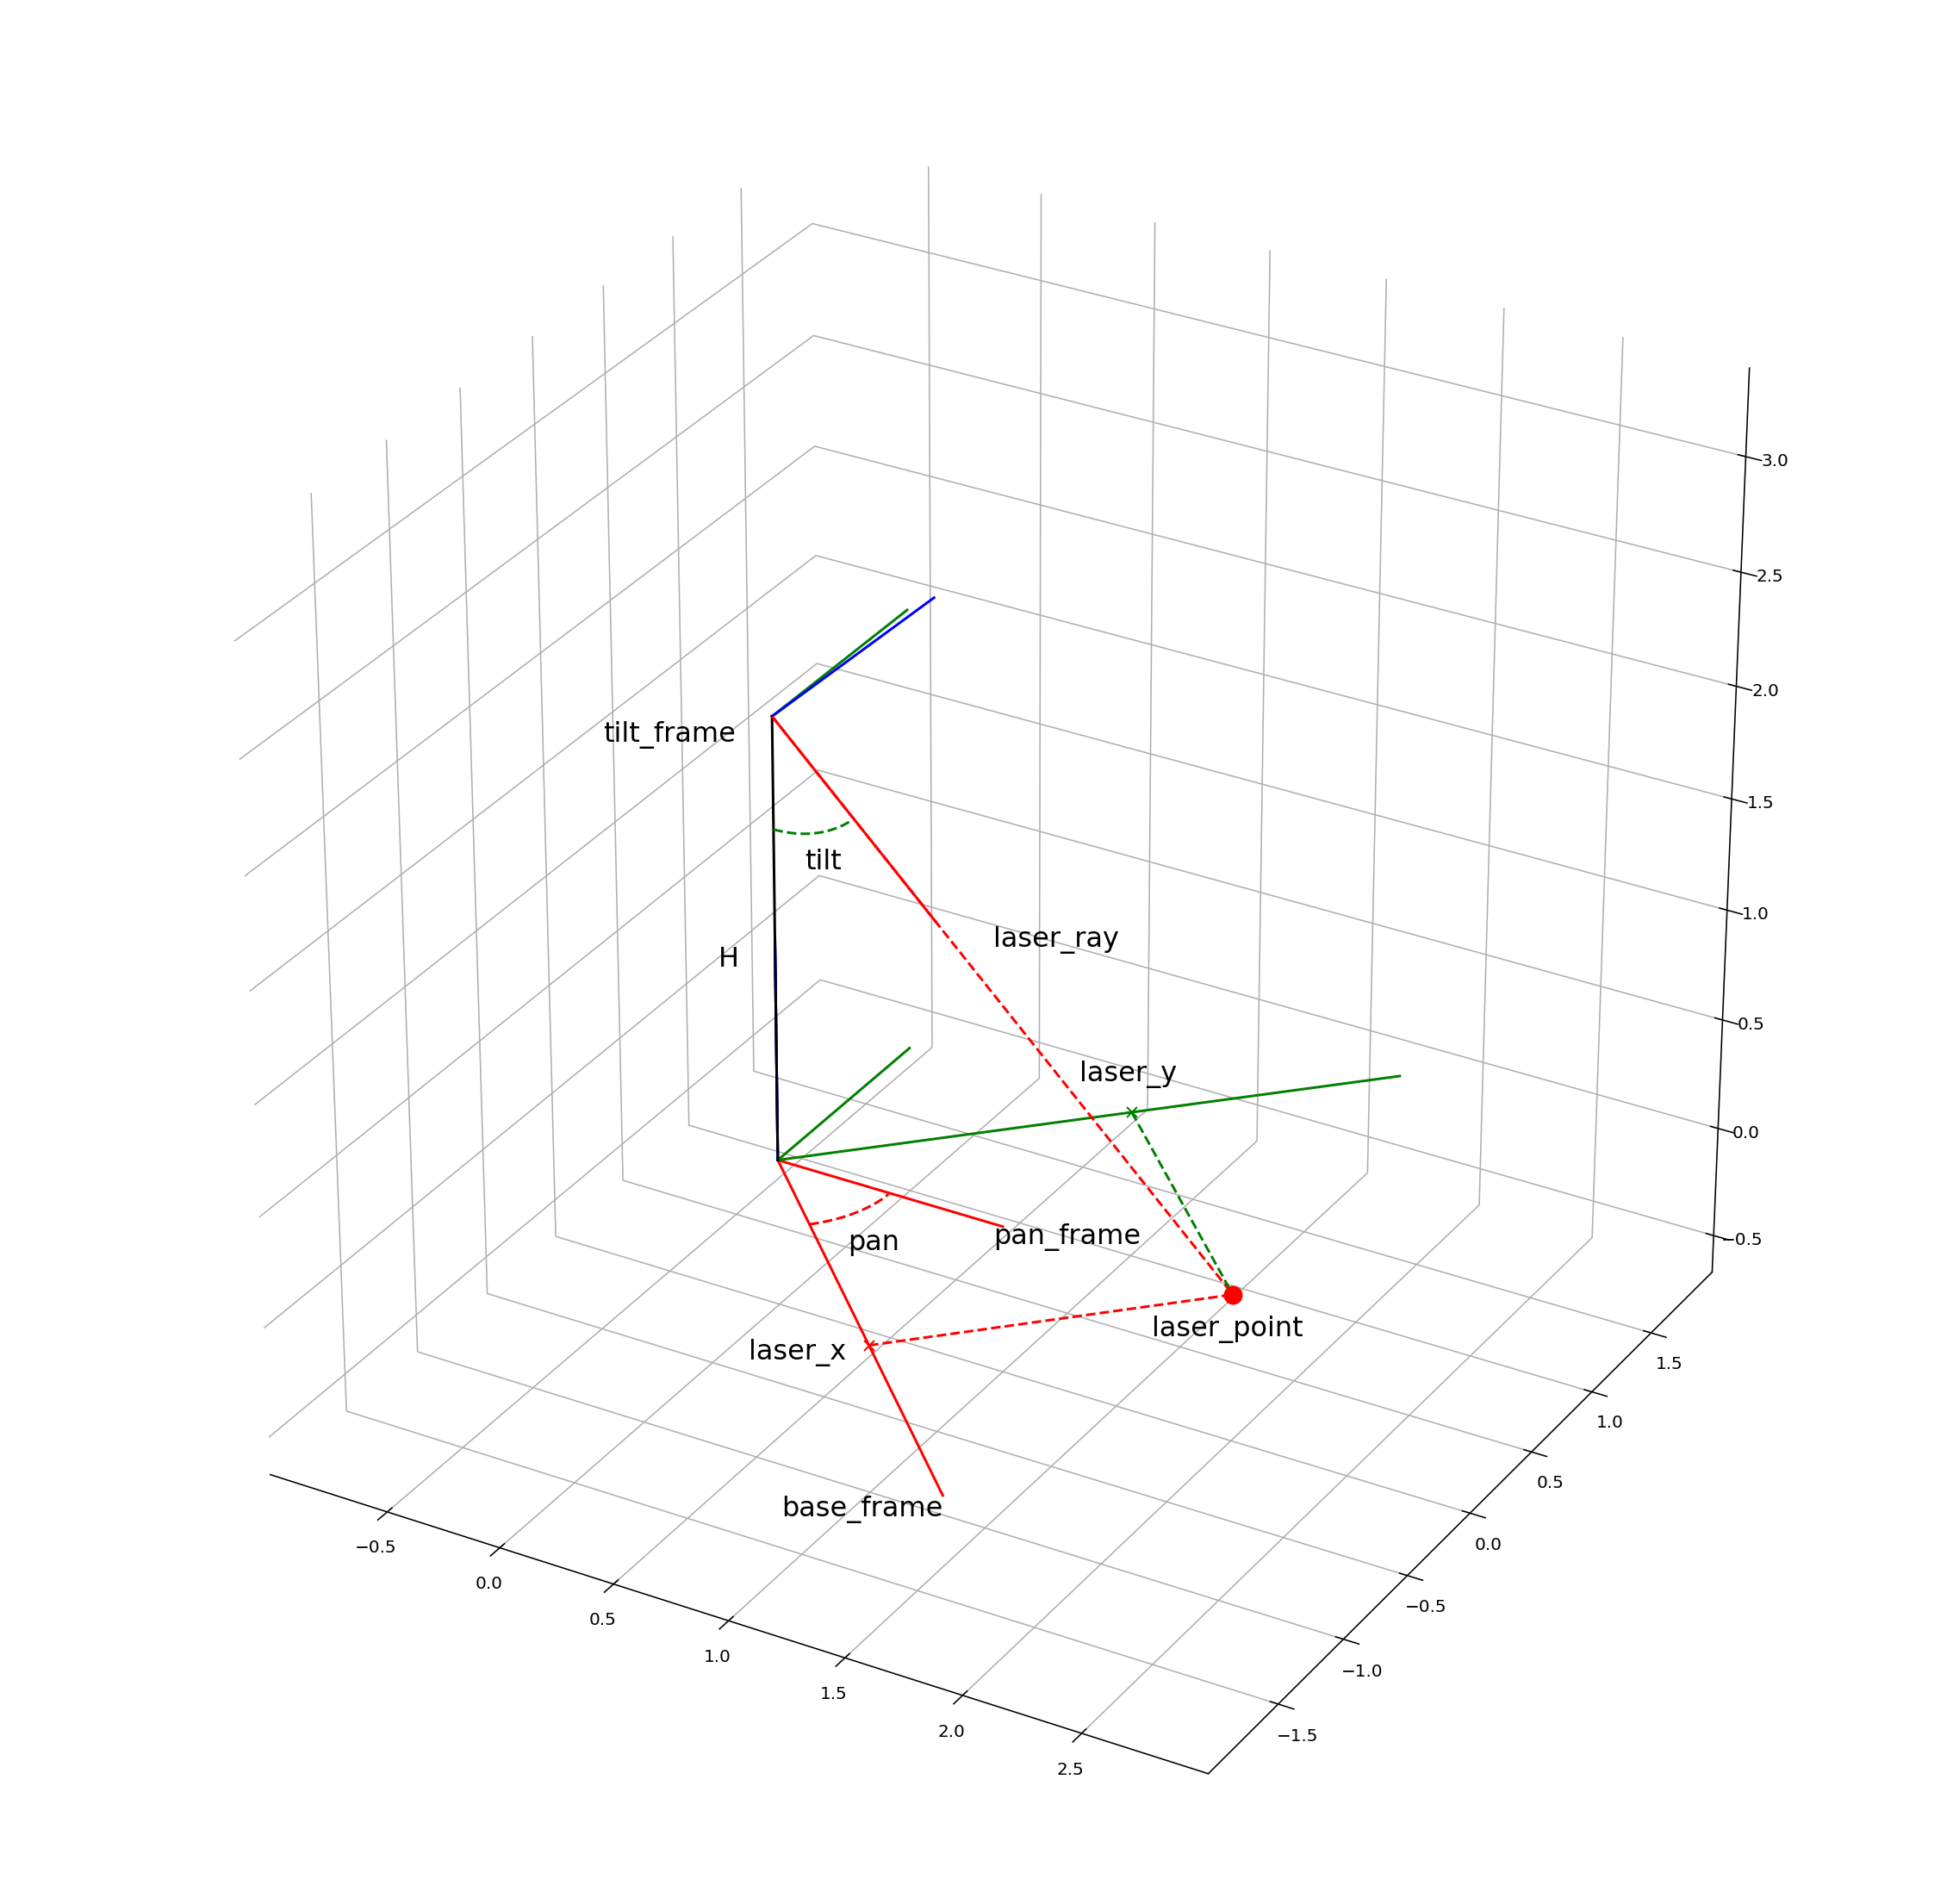
\includegraphics[width=\textwidth]{img/model1XY.png}%
	\caption{First Model, Pan \& Tilt Angle}
	\label{fig:firstModelPanTilt}
\end{figure}
\subsubsection{Inverse Kinematic}
The inverse kinematic takes as input the triple (\textit{x, y, z}) of the laser point and returns the corresponding \textbf{pan} and \textbf{tilt} angles.\\
In addition to \ref{eq:d}, we can say that:
\begin{align}
    H-z =& D\cos(tilt)\\
	L =& D\sin(tilt) \label{eq:dsin}\\
	L=& \sqrt{x^2+y^2}
\end{align}
Thus, we have that:
\begin{align}
    tilt =& \arctan\bigg(\frac{L}{H-z}\bigg) \label{eq:tiltik}\\
\end{align}
Finally, thanks to equations \ref{eq:x} and \ref{eq:y} we can immediately obtain:
\begin{align}
	pan=& \arctan\bigg(\frac{y}{x}\bigg)\label{eq:panik}
\end{align}
\\
\subsection{Second Model} \label{subs:secondModel}
The second model is slightly different from the first, as we can see in figure \ref{fig:secondModelRefFrame}. In that case, we have the laser ray which is perpendicular to the x axis of the \textbf{tilt\_frame}. One could think that to solve the inverse kinematic, adding 90 degrees to the tilt angle could be enough. However, since the ray origin does not coincide with the origin of the frame, this is wrong. Changing the tilt angle will not change only the direction of the ray, but also the position of its origin. This makes the kinematic a bit more complicated for that model.
\\
Here we report only the inverse kinematic as it is the most interesting to understand. Note that the assumption made for the \textit{z} of the laser point in section \ref{subs:firstModel} still holds.

\begin{figure}
	\centering
	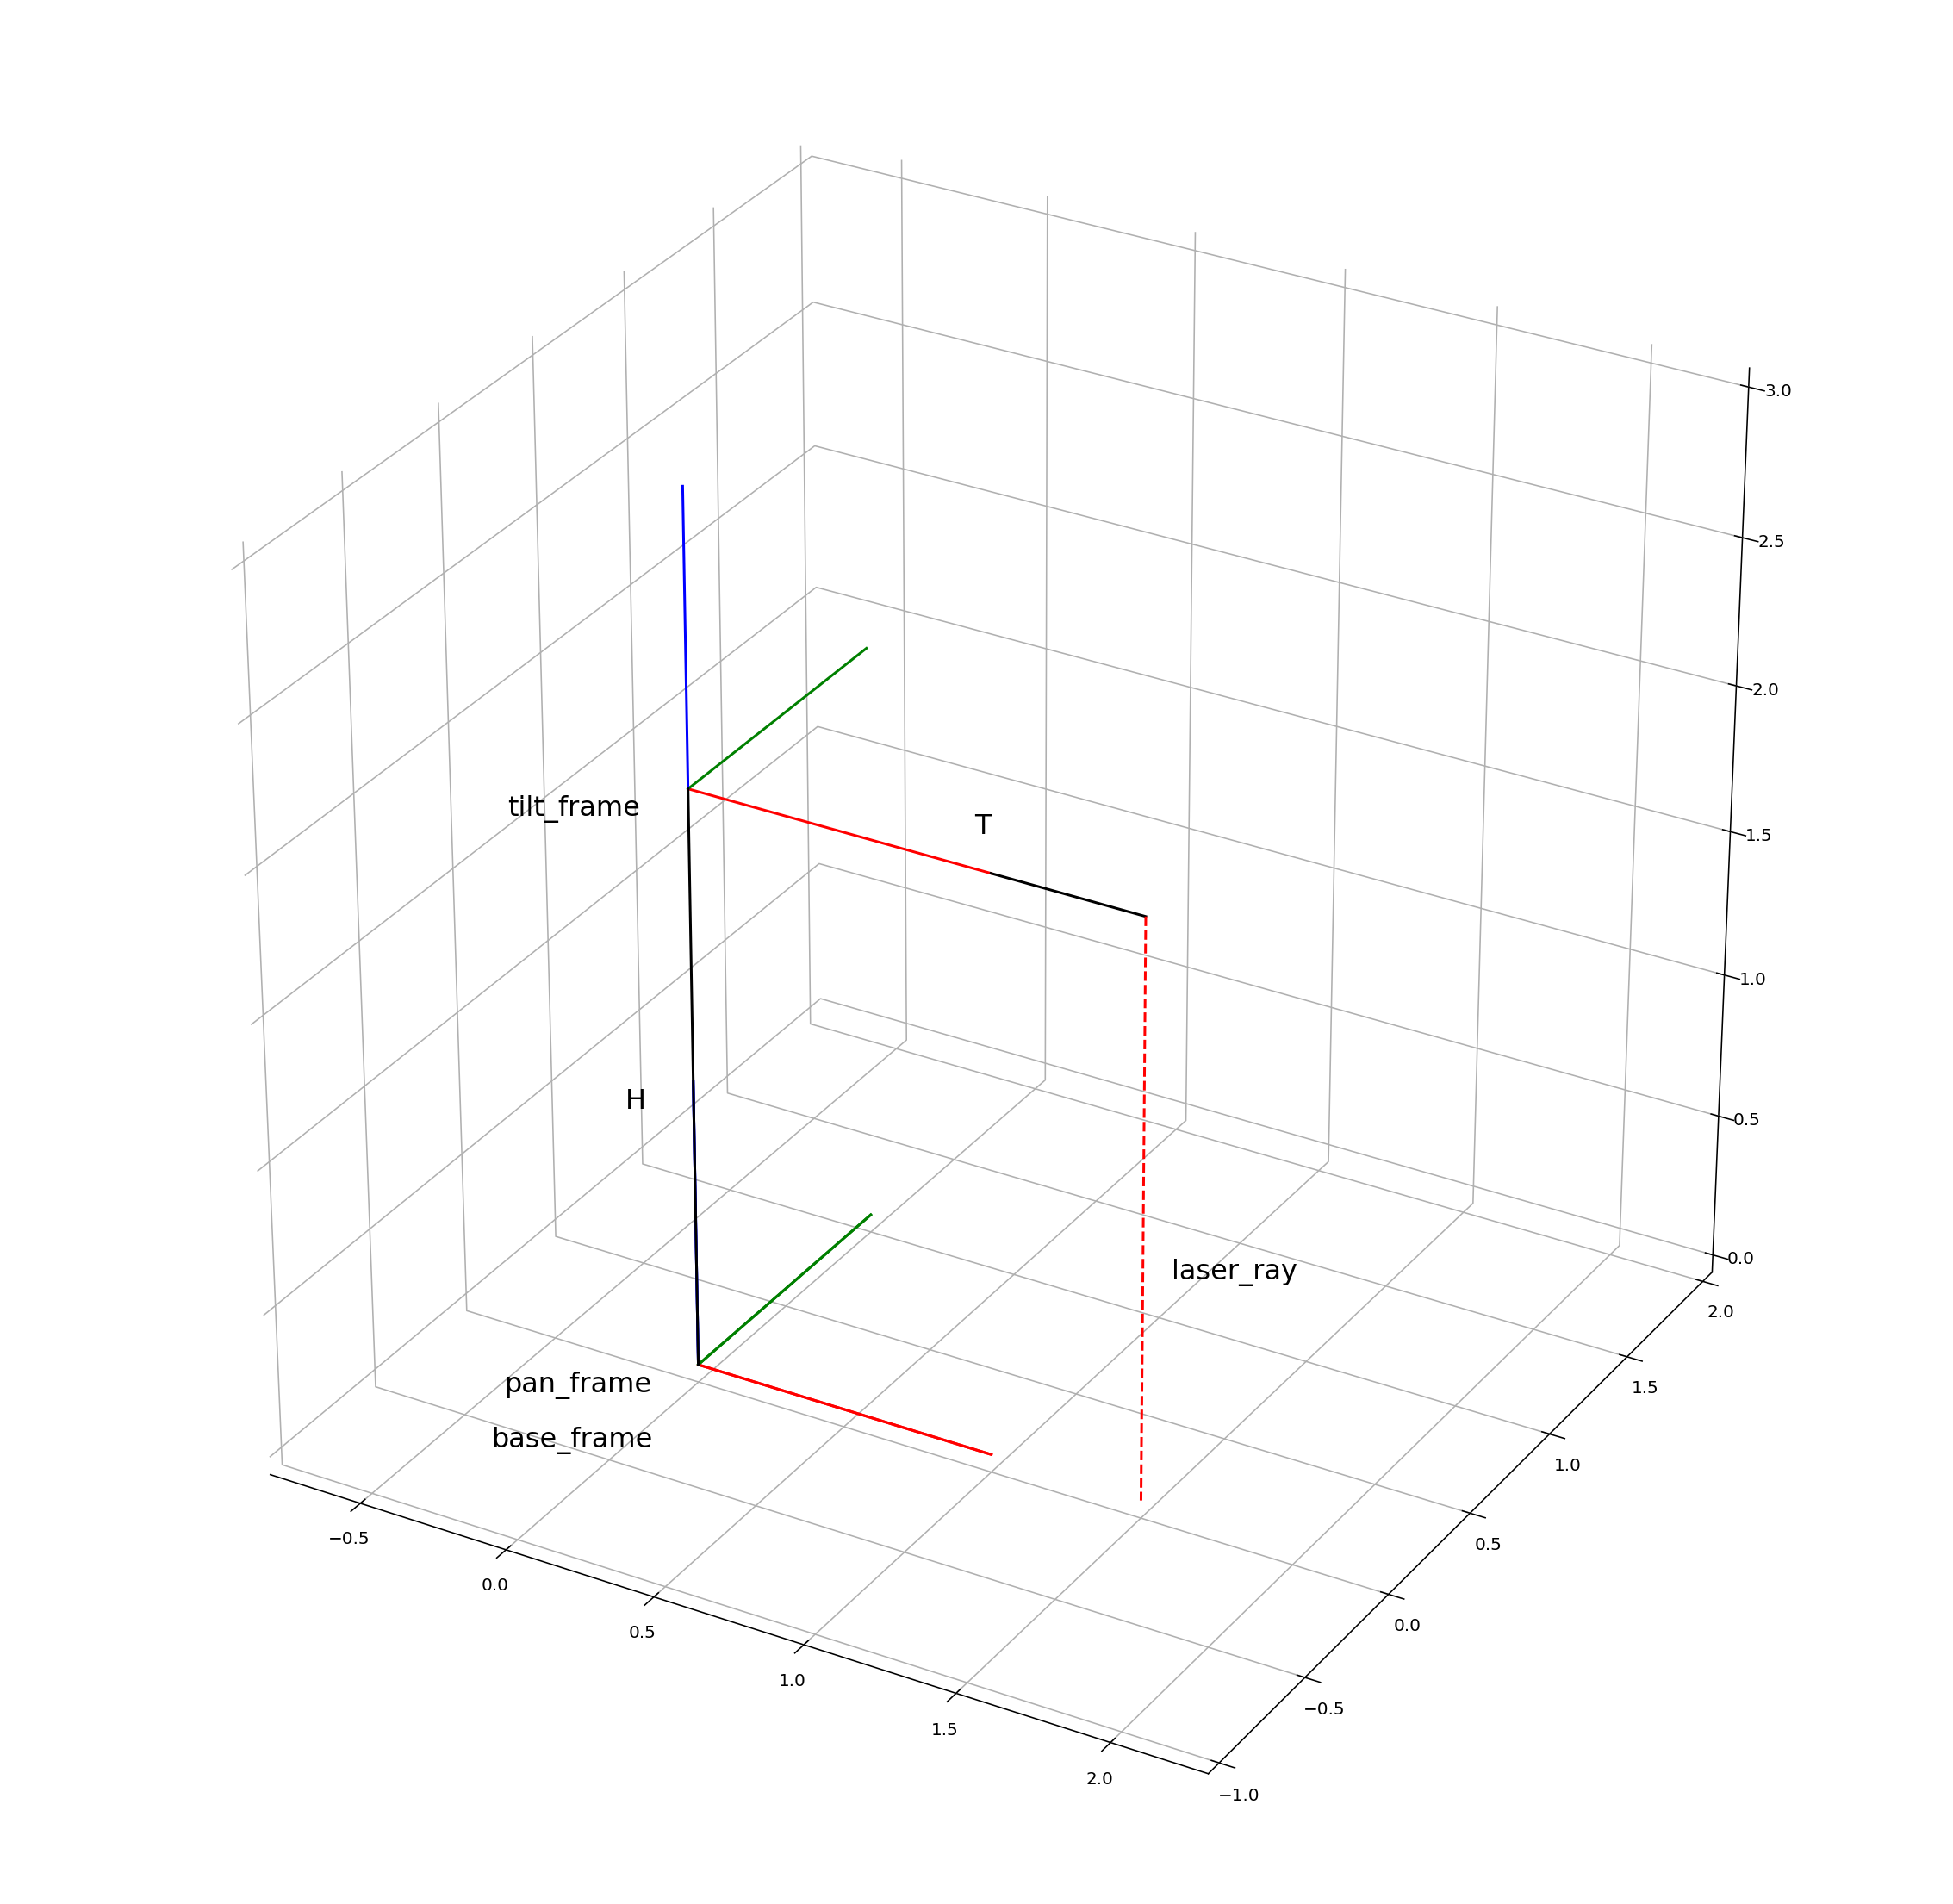
\includegraphics[width=\textwidth]{img/secondModel.png}%
	\caption{Second Model, Reference Frames}
	\label{fig:secondModelRefFrame}
\end{figure}

\subsubsection{Inverse Kinematic}
\begin{figure}
	\centering
	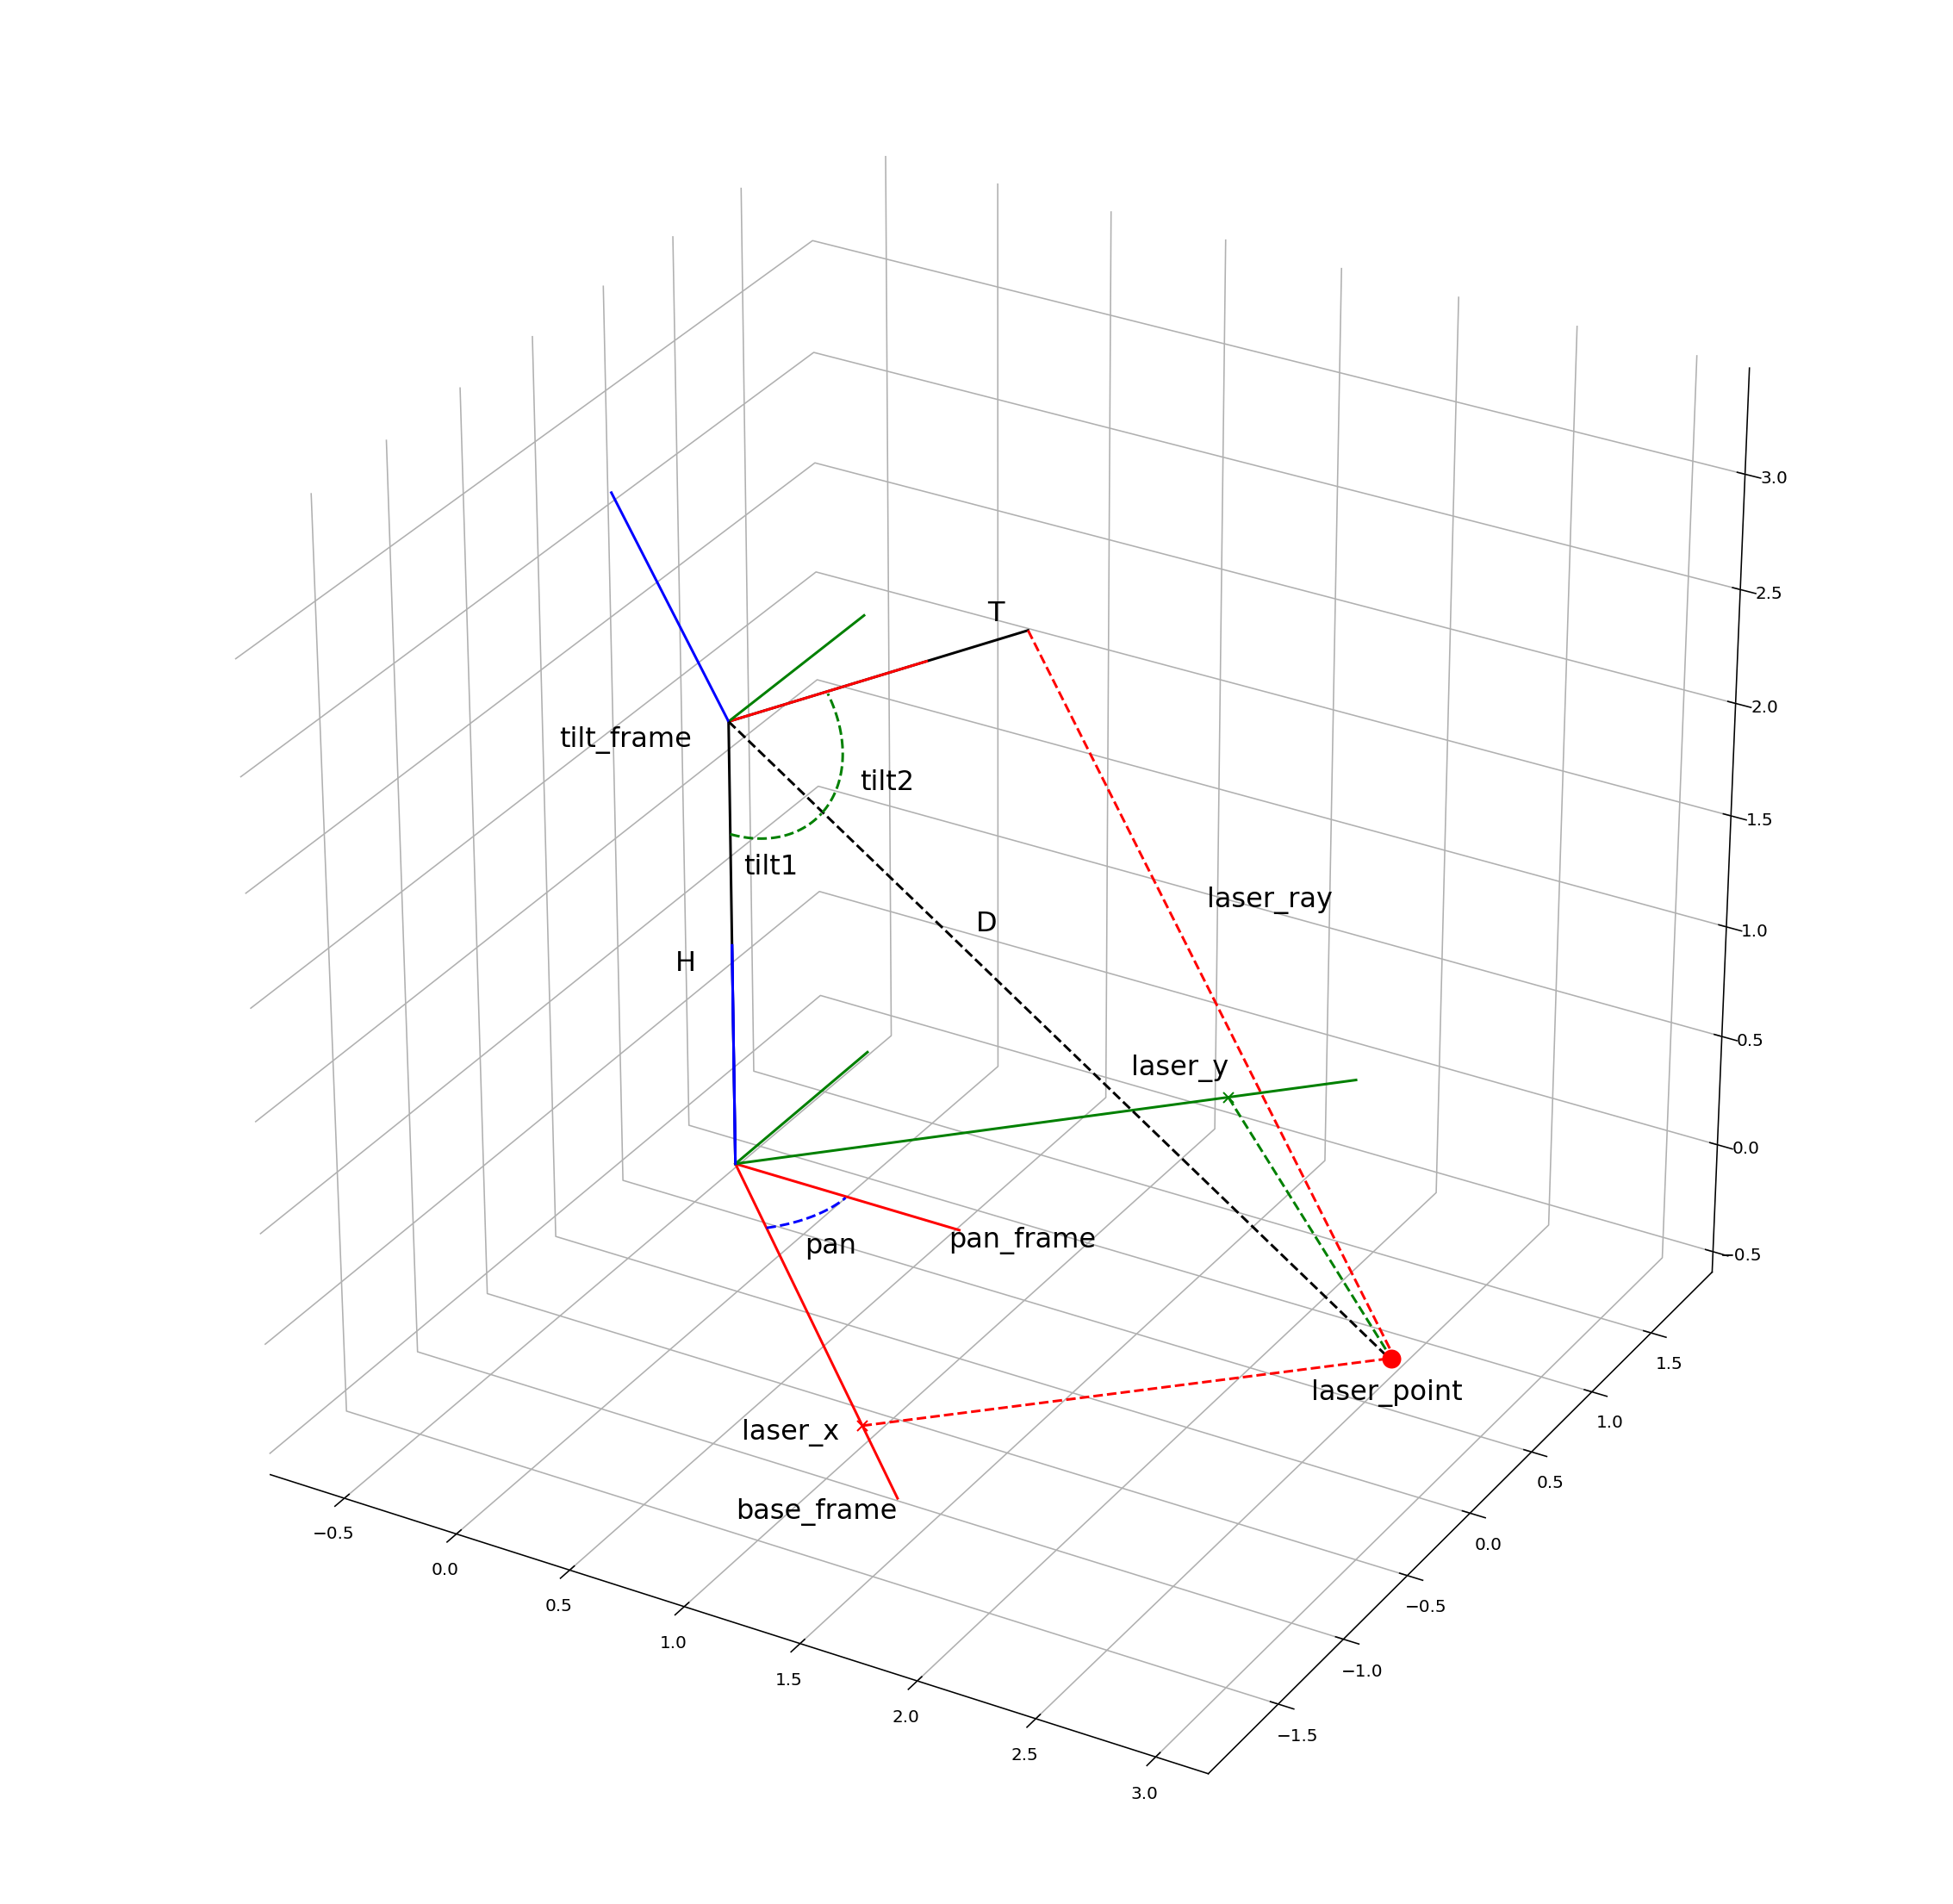
\includegraphics[width=\textwidth]{img/model2XY.png}%
	\caption{Second Model, Pan \& Tilt}
	\label{fig:secondModelPanTilt}
\end{figure}
First, we recall \textbf{L}, \textbf{D} and we introduce \textbf{T}:
\begin{itemize}
    \item \textbf{L} as the distance from the \textbf{pan\_frame} origin to the projection of the laser point on the \textbf{base\_frame};
    \item \textbf{D} as the distance from the \textbf{tilt\_frame} origin to the laser point;
    \item \textbf{T} as the known distance from the \textbf{tilt\_frame} origin to the laser ray origin.
\end{itemize}
As we can see in figure \ref{fig:secondModelPanTilt}, we have to decompose \textbf{tilt} in two parts, this is why we explicitly draw \textbf{D} that time. On the contrary, \textbf{pan} is obtained in the same way we did for the first model, thus:
\begin{align}
	pan=& \arctan\bigg(\frac{y}{x}\bigg)\label{eq:panik2}
\end{align}
Then we compute \textbf{L} and \textbf{D}:
\begin{align}
	L=& \sqrt{x^2+y^2}\\
	D=& \sqrt{(H-z)^2 + L^2}
\end{align}
Finally,
\begin{align}
	tilt1 =& \arctan\bigg(\frac{L}{H-z}\bigg)\\
	tilt2 =& \arctan\bigg(\frac{D}{T}\bigg)\\
	tilt =& tilt1 + tilt2
\end{align}
\\
\section{Human Pointing Model} \label{sec:1.2}
The approach we follow to model human pointing is the one used in \cite{gromov2018robot}. \\
The \emph{head-finger} model defines human pointing rays as originating at a centroid of the head and passing through the index fingertip. Figure \ref{fig:pointingModel} shows the model. \\
The reference frame \textbf{human\_footprint} is located at the human feet with the \emph{x}-axis pointing forward, \emph{y}-axis to the left, and \emph{z}-axis pointing up. The pointing ray is a 3D half-line on which the point that the human intends to indicate lies. So, our goal is to intersect that line with the floor (i.e. the \emph{xy}-plane of \textbf{human\_footprint} frame) in order to get the point indicated by the user. To do so, we get pointing rays using orientation readings from a wearable IMU. Once we have that, we can compute the intersection of those rays with the ground as a simple \emph{line-plane} intersection, as explained in \cite{O'Rourke:1998:CGC:289380}.
\\

Consider a line \textbf{L} given by its parametric equation:
\begin{align}
	P(s)= P_0 +s(P_1-P_0)= P_0+s\textbf{u}
\end{align}
where the parameter \emph{s} is a real number and $u=P_1-P_0$ is a line direction vector. Then, given a plane \textbf{P} expressed by a point $V_0$ on it and a normal vector $\textbf{n}=(a,b,c)$, we must first check if \textbf{L} is parallel to \textbf{P} by testing if $\textbf{b}\cdot\textbf{u}=0$, which means that \textbf{u} is perpendicular to \textbf{n}. In that case, \textbf{L} and \textbf{P} are parallel and thus either never intersect or else \textbf{L} lies completely on plane \textbf{P}.\\
If the line and the plane are not parallel, then we can compute their unique point intersection. Considering $\textbf{w} = P_0-V_0$, at the intersect point, the vector $P(s)-V_0=\textbf{w}+s\textbf{u}$ is perpendicular to \textbf{n}. This is equivalent to say that the dot product:
\begin{align}
	\textbf{n}\cdot(\textbf{w}+s\textbf{u})=0 \label{eq:dot}
\end{align}
Solving \ref{eq:dot} we obtain the intersect point $P(s_I)$:
\begin{align}\label{eq:intersection}
	s_I = \frac{\textbf{-n}\cdot\textbf{w}}{\textbf{n}\cdot\textbf{u}}=\frac{\textbf{n}\cdot(V_0-P_0)}{\textbf{n}\cdot(P_1-P_0)}=\frac{-(ax_0+by_0+cz_0+d)}{\textbf{n}\cdot\textbf{u}}
\end{align}
\begin{figure}
	\centering
	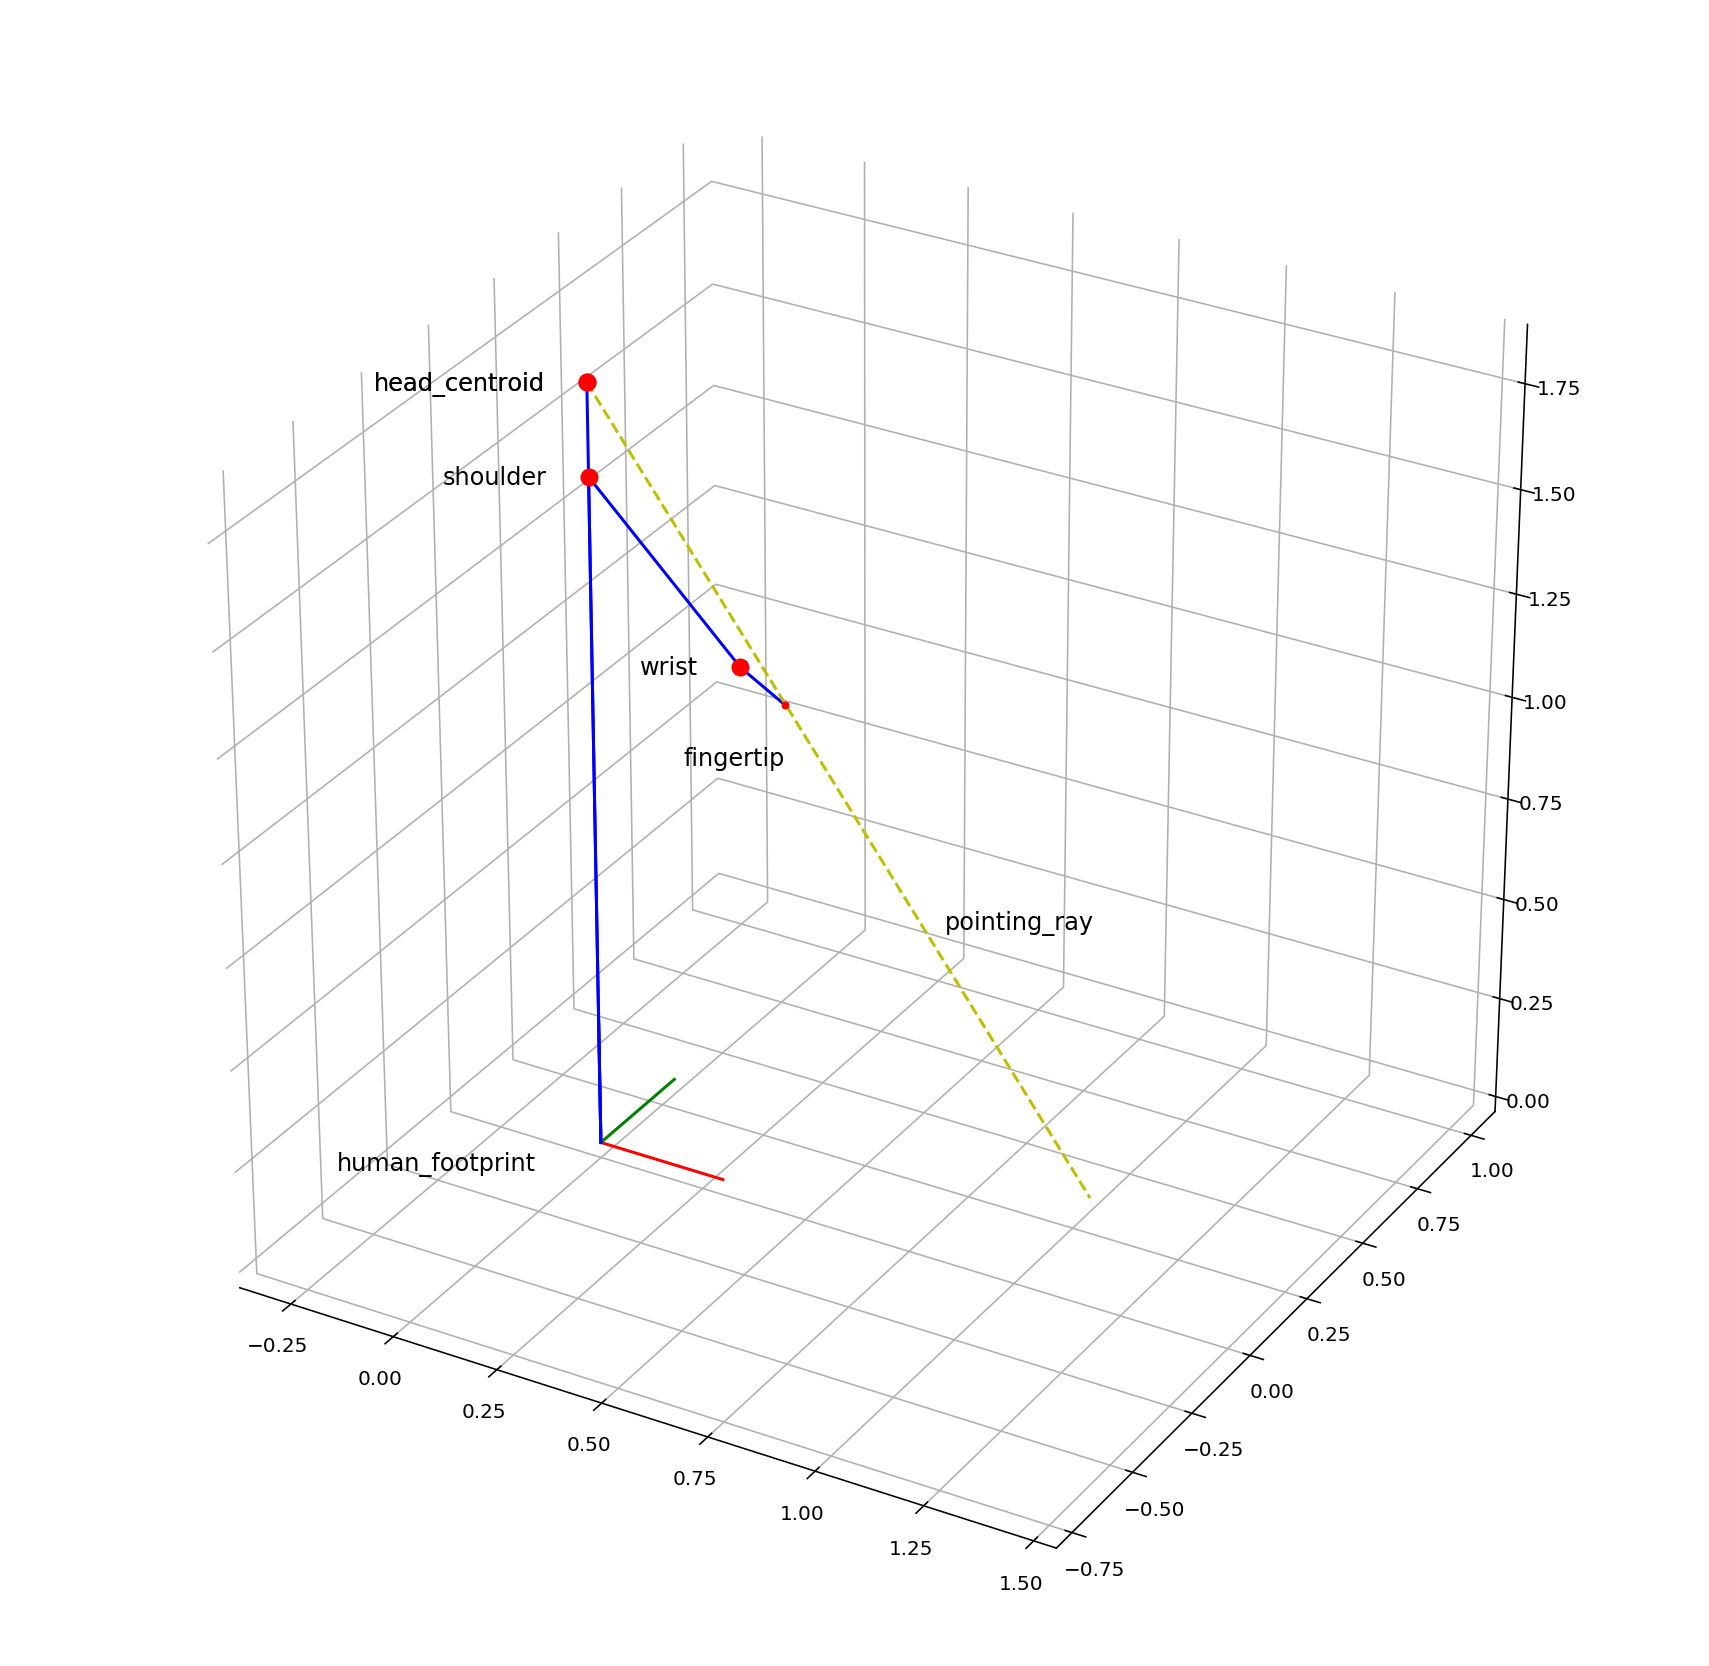
\includegraphics[width=\textwidth]{img/pointingModel.png}%
	\caption{Human Pointing Model}
	\label{fig:pointingModel}
\end{figure}
\section{Relative Localization} \label{sec:relloc}
The relative localization procedure goal is to estimate the pose (position and orientation) of the turret's frame in the reference frame of the human. The approach we use is the one proposed in \cite{gromov2018robot}.\\
First, we define the human frame $\{H\}$ the same way we did in section \ref{sec:1.2}. The reference frame $\{B\}$ is an arbitrary fixed reference frame in which the turret reports the position of the laser projected dot (in section \ref{sec:1.1} this is the \textbf{base\_frame}).\\ The input of the procedure is a finite set of pairs $C$:
\begin{align}
    C=\{(r_1^{\{H\}},P_1^{\{B\}}), \dots,(r_N^{\{H\}},P_N^{\{B\}})\}\nonumber
\end{align}
where $r_i^{\{H\}}$ is a pointing ray in the reference frame $\{H\}$ and $P_i^{\{B\}}$ is the corresponding laser dot position in the frame $\{B\}$. Those pairs are built collecting user's rays while he is following the moving laser with a pointing gesture for a short period of time $\tau$.\\
The output of the procedure is a coordinate transformation $T^*$ between the two frames, expressed as a composition of translation and rotation: 
\begin{align}
	\rho = [t_x, t_y, t_z, \gamma_z] \nonumber
\end{align}
where $t=[t_x, t_y, t_z]$ represent the translation, $\gamma_z$ the rotation around the \emph{z}-axis. Note that we simplify the model ignoring rotations around \emph{x}(roll) and \emph{y}-axis (pitch)  since the \emph{z}-axes of the user and the turret are parallel being both on the same plane (i.e. the floor).\\ Finding $\rho$ will allow us to collocate the turret's frame pose (position and orientation) into the human's frame.\\
This coordinate transformation is obtained through an optimization procedure: given an estimate $T$ of the transformation, we can convert laser positions $P_i^{\{B\}}$ defined in the turret frame into the operator frame:
\begin{align}
	P_i^{\{H\}}= TP_i^{\{B\}} \nonumber
\end{align}
Using these points we define a new ray $q_i^{\{H\}}$ that shares the origin with $r_i^{\{H\}}$, but passes through the point $P_i^{\{H\}}$. In that way we can define an error function $\theta$ for a set of pairs $C$:
\begin{align}\label{eq:error}
	\theta(T,C)=\frac{1}{N}\sum_{i=1}^N\angle(r_i^{\{H\}},q_i^{\{H\}})
\end{align}
where $\angle(\dots$) represents the unsigned angle between the directions of two rays. So, the goal of the optimization procedure is to find the coordinate frame transformation $T^*$ between the operator frame $\{H\}$ and the laser frame $\{B\}$ that minimizes that error function:
\begin{align}
	T^*=\argmin_T\theta(T,C)
\end{align}
